\documentclass[11pt, onehalfspacing]{article}
\usepackage[margin=2cm]{geometry} % page margin
\usepackage{lineno} % line numbers
\usepackage{graphicx} % importing plots
\usepackage{fancyhdr}
\usepackage{natbib}
\usepackage{float}

\usepackage{rotating}

\title{Project Proposal}	% Title
\author{David Scott}			% Author
\date{March 2019}			    % Date

\makeatletter
\let\thetitle\@title
\let\theauthor\@author
\let\thedate\@date
\makeatother

\pagestyle{fancy}
\fancyhf{}
\rhead{\theauthor}
\lhead{\thetitle}
\cfoot{\thepage}

\usepackage{xcolor}
\usepackage{colortbl}

\usepackage{forloop}
\newcounter{loopcntr}
\newcommand{\rpt}[2][1]{%
	\forloop{loopcntr}{0}{\value{loopcntr}<#1}{#2}%
}
\newcommand{\on}[1][1]{
	\forloop{loopcntr}{0}{\value{loopcntr}<#1}{&\cellcolor{gray}}
}
\newcommand{\off}[1][1]{
	\forloop{loopcntr}{0}{\value{loopcntr}<#1}{&}
}

\usepackage[utf8]{inputenc} % set input encoding to utf8
\usepackage{booktabs}
\usepackage{longtable}

\newcommand{\done}{\cellcolor{teal}done}  %{0.9}
\newcommand{\hcyan}[1]{{\color{teal} #1}}


\begin{document}
	\begin{titlepage}
	\centering
	\vspace*{0.5 cm}
	
\includegraphics[scale = 0.15]{logo2.png}\\[1.0 cm]	% University Logo
	\textsc{\LARGE Development of microbial population dynamics models from omics data}\\[1 cm]
	\textsc{\Large David Scott}\\[0.5 cm]
	\textsc{\Large Computational Methods in Ecology and Evolution (MSc)}\\[0.5 cm]				% Course Code
	\textsc{\Large Imperial College London}\\[0.5 cm]
	\rule{\linewidth}{0.2 mm} \\[0.4 cm]
	{ \huge \bfseries \thetitle}\\
	\rule{\linewidth}{0.2 mm} \\[0.75 cm]
	\textsc{\Large Supervisor: Dr. Alberto Pascual--Garcia}\\[0.5 cm]	
	\textsc{\Large Affiliated Institute: ETH Zurich}\\[0.5 cm]
	\textsc{\Large Email: alberto.pascual@env.ethz.ch}\\[0.5 cm]		
	\vspace*{2 cm}
	\begin{minipage}{0.4\textwidth}
		\begin{flushleft} \large
			\emph{Submitted To:}\\
			Dr. Samraat Pawar\\
			Course Director\\
		\end{flushleft}
	\end{minipage}~
	\begin{minipage}{0.4\textwidth}
		
		\begin{flushright} \large
			\emph{Submitted By:} \\
			David Scott\\
			01602669\\
		\end{flushright}
		
	\end{minipage}\\[2 cm]
	
\end{titlepage}

\textbf{Keywords:} Microbial Communities, Metabolics, Modelling, Genomics, Population Dynamics, ODE. 

\section{Introduction}
The role played by microbial communities has been increasigly recognised and has attracted much attention across disciplines from soil ecology \citep{torsvik2002microbial} to the human microbiome \citep{ley2008worlds} and biotechnological processes \citep{rabaey2004biofuel}. These roles or ecological functions are not the product of, or characteristics of, an individual species or process, but of the community as a whole. 

Microbes alter the biochemistry of their media by metabolising a resource and outputting a by product, which in many cases can too be a resource. Thus, the consequence of the co-occurance of species under constant environmental conditons is not limited to competition (two species sharing same reseource). Cooperation  or metabolic complementarity (metabolites of one species consumed by another) enables communties to shape their own niche, promoting community stability \citep{freilich2011competitive}. Therefore the combined metabolisms of individual member species create the community metabolome which determines the ecological function (\citep{arrigo2004marine}; \citep{goodman2010our}; \citep{noecker2016metabolic}).

Hence, to understand the organisational principles that determine the behaviour of communities a mechanistic understanding of interspecies interactions is required \citep{henry2016microbial}. However, little is known about the processes that determine the assembly and function of these microbial communities. It is difficult to investigate functions due to the diversity of species in natural communtiies, and isolating them to an axenic culture. A solution to this problem is to identify combinations of species abundances within stable communities compatable with the observation of the function of interest (Figure \ref{fig1}).  

%stoichioemtry - based metabolic models have shown accurate predictions for the patterns of metabolic interactions in bacterial two species systems. 

%bottom up approximations such as flux balance analysis aim to create a metabolic model for each individual species, emcompassing its uptake and secretion of metabolites, and then adding comlexity by increasing the number of species. This lacks when multiple spcies are added due to the increase in interactions, which is the case in eal life scenarios. [35]

%top down approximation ossible to predict mc states without accurate individual species models. As some secies ssytematically co exist due to either similar environmental preferences or reciprocal influence. Uses data from high throughput NGS experiments to relate microbial cmposition with species interactions. Some approx aim to predict cmmunity metabolome from info provid by its metagenome. 

%experiments analysing growth of natural communities report a systematic convergence to the same steady states [58] fig 1


The aim of this project will be to explore different strategies to develop population dynamics models of microbial communties from empirical data. Through combining 16S rRNA, metagenomics and metabolomics data, we aim to infer ecological interactions and trophic strategies, from the analysis of both the abundances of species and their genetic repertoires. There are two data sets available to the study. The first dataset consists of assemblage experiments of marine particles data on pure polymer substrates, spanning 200h (12 time points), and includes both 16S rRNA and metagenomics data (Prof. Otto Cordero lab. \citep{datta2016microbial}). The second dataset contains ~700 16S rRNA samples of beech tree-holes, a natural aquatic habitat, and of a second subset of 250 samples of the same communities grown in the lab for seven days (Prof. Thomas Bell lab). For this new dataset, 16S rRNA and functioning of the communities was measured. 

\begin{figure}[H]
	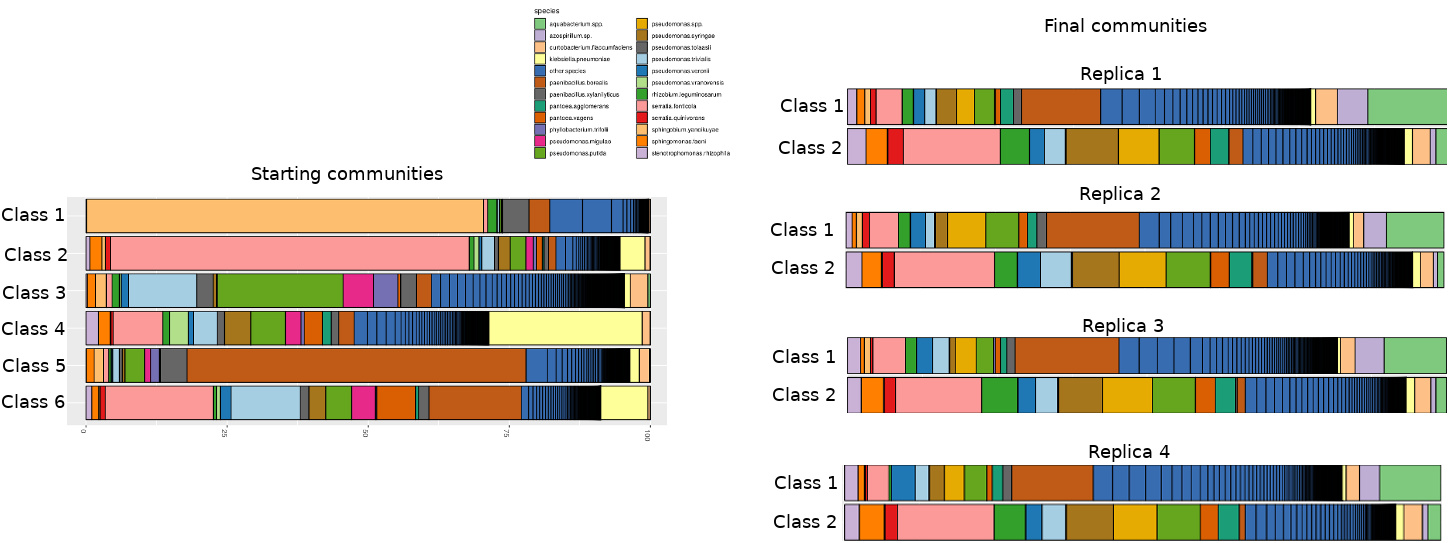
\includegraphics[width=\linewidth]{figure1.png}
	\caption{The 700 communties sampled from beech tree holes were classified into six classes (left panel). The size of each bar represents the relative abundance of OTU's. These are groups of species with 97\% similarity. A subset of 250 microbial communities comprising of all six classes were then regrown under laboratory conditions. The final communites could be classified into two classes, with striking similarity between the four replicates (right panel).}
	\label{fig1}
\end{figure}

%Although the first dataset is richer and contains metagenomic data, the second dataset is more reproducible. A subset of 250 samples was further grown in the laboratoryWhile they will be limited in data point (12 and 2 respectively) there are reproducible trajectories. Will explore either metabolic models (marine particles data) or with functionality (beach tree data). Different states will be explored with ordinary differential equations (ODE). 



\section{Proposed Methods}

%In this project, it will be explored 

%It is hoped to develop the ability to explore the different tools and  ordinary differential equation population dynamic models for this task. 

Despite of the complexity of the dataset, the reproducibility of the experiments is quite remarkable (see Figure \ref{fig1} \& \ref{fig2}). Given this reproducibility, I aim to parameterize population dynamics models following different strategies. The main rational behind the strategy is that it may be possible to infer interactions from correlations between either abundances, genes or both. Therefore, the first part of the project will attempt to infer networks of putative interactions, reducing its complexity with network analysis and studying if it is possible to interpret network motifs ecologically. This would allow us to build models of Lotka-Volterra type (\citep{allesina2012stability}; \citep{taillefumier2017microbial}; \citep{marsland2019available}) where the information about the interplay between species and resources is kept implicit. For this task, the beech-tree dataset will be used.

A second approximation consists of predicting the underlying resources underlying the population dynamics. Starting from the metagenomics information, we aim to infer community-level metabolic networks as outlined by \citep{henry2016microbial}. In addition, if metabolomics data is available, metagenomics composition can be linked with the underlying resources \citep{noecker2016metabolic}. We will make this prediction for each time point of the marine particles data, for which metabolomics information is available. Then, we will analyse the dynamics of resources looking for correlations, as it was done in the previous task. Combining the network of resources and the one of species abundances, we will attempt to parameterize population dynamics models with both resources and consumers explicit (\citep{marsland2019available}; \citep{taillefumier2017microbial} \citep{posfai2017metabolic}; \citep{goyal2018diversity}; \citep{tikhonov2017collective}). 

\begin{figure}[H]
	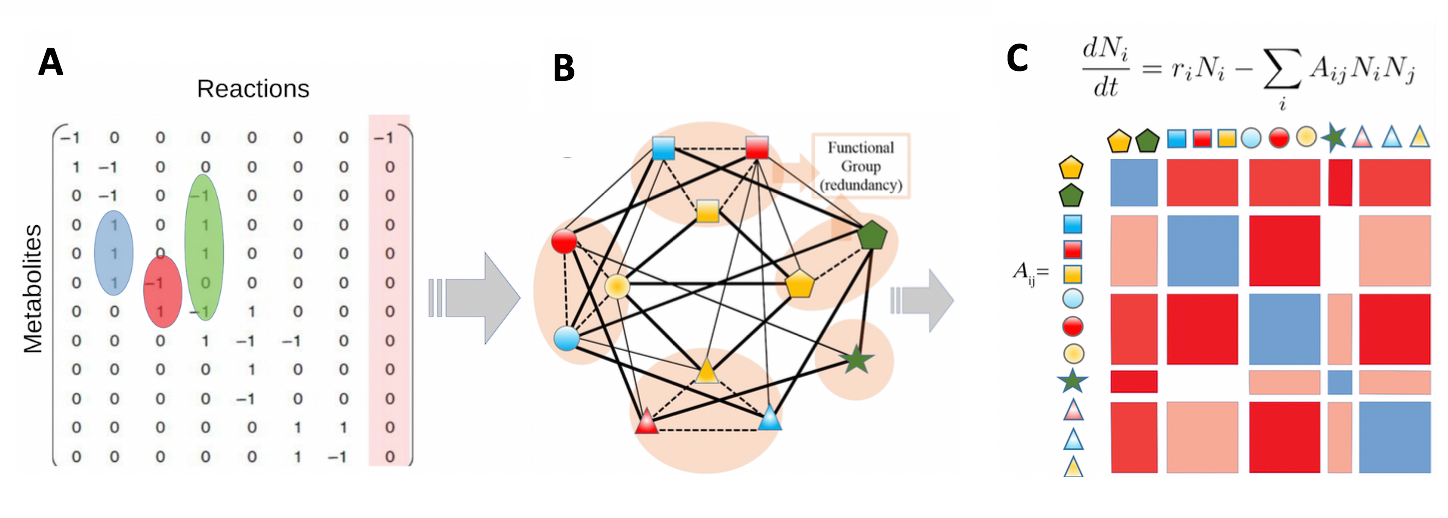
\includegraphics[width=\linewidth]{figure2.png}
	\caption{A) Community level metabolic matrix of the contribution of each species. B) Shape's represent unique species contributions. These are used in large communities, identify those with the same contribution to determine functional groups. C) An interaction matrix (A$_{ij}$) represents this analysis with competition within functional groups in blue and cooperation between them in red.}
	\label{fig2}
\end{figure}

%There are two datasets available to the study. The first, marine particles set, consists of 16S RNA (8 substrates and 12 time points) metagenomics and isolates (~1000, 60 of them with the whole genome sequenced). Therefore there are species with known metabolisms and thus individual metabolic models can be built from the whole sequenced genomes using flux balance analysis \citep{orth2010flux}. This data will be aquired from Dr. Otto Cordero \citep{datta2016microbial}. Community level metabolic networks can be constructed from these individual models or modelled as outlined by \citep{henry2016microbial}. Once community metabolisms are modelled it is hoped to then use ODE to infer population dynamics. There is also potential to incorporate the substrate into the model. 

%The second, consists of microbial communities collected from pools of water at the buttress of beech tree roots. This data consists of four replicates of each community.  It is limited to two data points, the initial state and the state after seven days. It contains more species that the marine particles, but lacks any sequenced whole genomes. However, many of the species present are also present in the human microbiome so metabolic models for individuals may be aqcuired, from which a community level metabolic model could be constructed. This will be aquired from Dr. Tom Bell \citep{rivett2018abundance}. Alternatively the functionality of communities after seven days can be used. Statistical models could be combined to explore community functions or try a population dynamic approach.


\section{Outcomes}
This project will culminate in a report produced in the style of a scientific paper, in partial fulfillment of an MSc in Computational Methods in Ecology and Evolution at the Imperial College London. The findings of this project will be presented and defended in a viva during the month of September 2019. 

\newpage
\section{Project Timeline}

The project will run over a six month period beginning the 1st of April 2019 and ending the 28th of September 2019. I will be based in ETH Zurich for the months of May, June and July where I will work directly with my supervisor Dr. Alberto Pascual-Garcia. 

\bigskip

\noindent\begin{tabular}{p{0.17\textwidth}*{24}{|p{0.01\textwidth}}|}
\textbf{Gantt chart} 
& \multicolumn{4}{c|}{April} 
& \multicolumn{4}{c|}{May} 
& \multicolumn{4}{c|}{June} 
& \multicolumn{4}{c|}{July}
& \multicolumn{4}{c|}{August} 
& \multicolumn{4}{c|}{September} \\

\rpt[6]{& 1 & 2 & 3 & 4} \\
\hline
\textbf{The  \mbox{Project}} & \multicolumn{24}{c|}{} \\
\hline
% using the on macro to fill in cells as `on'
Project Proposal  \on[1] \off[23] \\
\hline
Review Methods    \on[4]  \off[20] \\
\hline
Model Metabs     \off[4] \on[4] \off[16] \\
\hline
Model Pop Dyns     \off[8] \on[4] \off[12] \\
\hline
Analyse Results     \off[12] \on[4] \off[8] \\
\hline
Literature    \on[20] \off[4] \\
\hline
% The mbox prevent packages from being hyphenated
% The multicolumn produces no vertical guides within the columns it spans, but
% does put one at the end to complete the righ-hand edge of the table
\textbf{The \mbox{Report}} & \multicolumn{24}{c|}{} \\
\hline
Introduction \on[12] \off[4] \on[4] \off[4] \\
\hline
Methods \off[4] \on[8] \off[12] \\
\hline
Results \off[12] \on[4] \off[8] \\
\hline
Discussion \off[14] \on[6] \off[4] \\
\hline
\textbf{The \mbox{Assesments}} & \multicolumn{24}{c|}{} \\
\hline
Submission  \off[19] \on[1] \off[4] \\
\hline
Presentation  \off[20] \on[4] \\
\hline
viva  \off[20] \on[4] \\
\hline

\end{tabular}

\section{Budget}
Costs calculated in pound sterling. Accomodation outlines the cost for three months accomodation in Zurich for the months of May, June and July 2019. Travel covers the cost a return flight. Mobility fund is 291.36 pounds contributed by the Swiss government each month I am there. This is part of the Swiss-European Mobility Fund. In total, a deficit of £1031 will be incurred.  

\bigskip




\begin{table}[H]
\begin{center}
	\caption{All expected expenses and income associated with the project. Currency is pounds Sterling. }
\begin{tabular}{lrr}
	\toprule
	Details      & Expense  & Income \\
	\midrule
	Accomodation    & 1705   &  \\                                                     
	Travel  & 200 & \\
	Mobility Fund  & & 874\\ 
	Course Budget  & & ??\\ 
	\hline
	Total & 1905 & 874 \\
	\bottomrule              
\end{tabular}
\end{center}
\end{table}


%\newpage
%\bibliographystyle{agsm}
%\bibliography{project_proposal}

%\newpage

%Primary Supervisor: Dr. Alberto Pascual Garcia \\

%Insitute: ETH Zurich \\

%\textbf{“I have seen and approved the proposal and the budget”} \\

%Signature: \\

%Date: \\

\end{document}

